\subsection{Deliverable capacity, channel price and coordination}
\label{sec:res-capacity-all}

\subsubsection{Reliably deliverable capacity and virtual--physical substitution}
\label{sec:res-capacity}

In the rule setting, each uniform commitment from 4 to 9~MW was run on 20 operating days in closed loop
(\tabref{tab:capacity}, \figref{fig:capacity}). Requiring all three events to be valid on at least 95\% of the days,
IR-O* can commit 6~MW, IR-P reaches this reliability at no commitment level, and JR-D can commit 8~MW, which is 33\%
more. At the respective best commitments, JR-D (7~MW, $18.89\times10^4$~CNY per day) is 4.1\% cheaper than IR-O* (6~MW,
$19.70\times10^4$~CNY per day).

\begin{table}[!t]
\caption{Closed-loop reliability by uniform commitment (rule setting, 20 days): share of days with all events valid /
mean total cost ($10^4$~CNY).}
\label{tab:capacity}
\centering\footnotesize
\begin{tabular}{@{}cccc@{}}
\toprule
Commitment (MW) & IR-O* & IR-P & \textbf{JR-D}\\
\midrule
4 & 75\% / 21.63 & 85\% / 21.42 & \textbf{100\% / 20.69}\\
5 & 80\% / 20.83 & 75\% / 21.05 & \textbf{100\% / 19.75}\\
6 & 95\% / 19.70 & 80\% / 20.27 & \textbf{100\% / 19.05}\\
7 & 80\% / 20.32 & 70\% / 20.34 & \textbf{95\% / 18.89}\\
8 & 50\% / 21.38 & 40\% / 21.65 & \textbf{95\% / 19.20}\\
9 & 25\% / 22.97 & 25\% / 23.42 & 65\% / 21.01\\
\bottomrule
\end{tabular}
\end{table}

\begin{figure*}[!t]
\centering
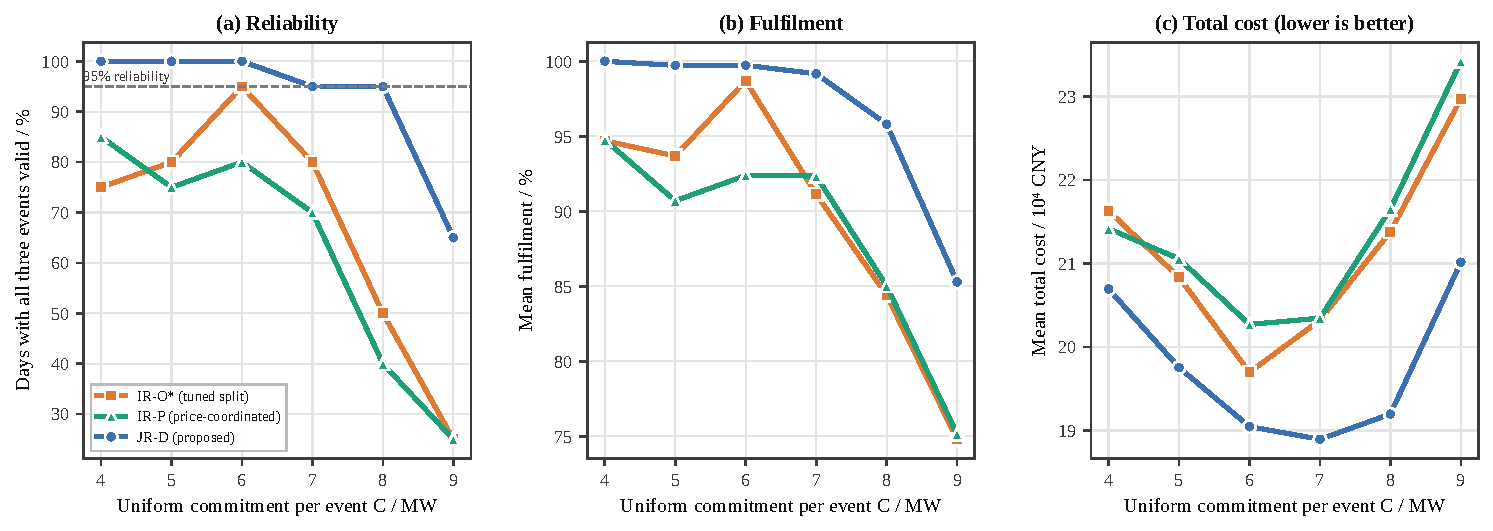
\includegraphics[width=0.94\textwidth]{fig11_capacity.pdf}
\caption{Closed-loop reliability, fulfilment and total cost versus the uniform commitment (rule setting, 20 operating
days).}
\label{fig:capacity}
\end{figure*}

The virtual--physical substitution experiment sweeps the BESS energy (at 6~MW power and a fixed absolute connection
limit) and the connection margin $\gamma$ under perfect information and finds the largest uniform commitment that is
fulfilled at $\ge$99\% with all events valid (\tabref{tab:subst}, \figref{fig:subst}). Joint recovery is worth about
9--12~MWh of battery: JR reaches 6.5~MW with a 3-MWh battery, which IR-O* needs 12~MWh for; JR reaches 7.0~MW with
6~MWh, which IR-O* needs 15--18~MWh for; and JR reaches 8.0~MW with 12~MWh, which independent recovery does not reach
with any battery size. Joint recovery is also worth about 2.9~MW of connection capacity: JR reaches 8.0~MW at
$\gamma=1.10$, whereas IR-O* needs $\gamma=1.30$, \ie\ $0.2\times14.57\approx2.9$~MW more; the 7.0~MW of JR at
$\gamma=1.00$ likewise requires $\gamma=1.20$ for IR-O*. At its reliable capacity, JR carries a long-lag backlog worth
6.0--7.0~MWh into E3, about half of the 12-MWh battery (\figref{fig:subst}(c)); the smaller the battery, the more this
virtual computing storage is used, and with 18~MWh or more the physical storage suffices and joint recovery no longer
needs it.

\begin{table}[!t]
\caption{Reliable uniform commitment (MW, $\ge$99\% fulfilment with all events valid, perfect information).}
\label{tab:subst}
\centering\footnotesize
\setlength{\tabcolsep}{3.6pt}
\begin{tabular}{@{}lccccccc@{}}
\toprule
BESS energy (MWh) & 3 & 6 & 9 & 12 & 15 & 18 & 24\\
\midrule
JR & 6.5 & 7.0 & 7.5 & \textbf{8.0} & 7.5 & 7.0 & 6.5\\
IR-O* (hindsight) & -- & 5.0 & 6.0 & 6.5 & 7.0 & 7.0 & 6.5\\
IR-P & -- & 5.0 & 5.5 & 6.0 & 5.0 & -- & --\\
Backlog carried into E3 by JR (MWh) & 6.8 & 7.0 & 7.0 & 6.0 & 3.5 & 0.8 & 0\\
\midrule
Connection margin $\gamma$ & 1.00 & 1.05 & 1.10 & 1.15 & 1.20 & 1.30 & \\
\midrule
JR & 7.0 & 7.5 & \textbf{8.0} & 8.0 & 8.0 & 8.0 & \\
IR-O* (hindsight) & 6.0 & 6.0 & 6.5 & 6.5 & 7.0 & 8.0 & \\
IR-P & 5.0 & 5.5 & 6.0 & 7.0 & 6.0 & 6.0 & \\
\bottomrule
\multicolumn{8}{@{}l@{}}{\scriptsize --: not reached within the sweep (5--9.5~MW).}
\end{tabular}
\end{table}

\begin{figure*}[!t]
\centering
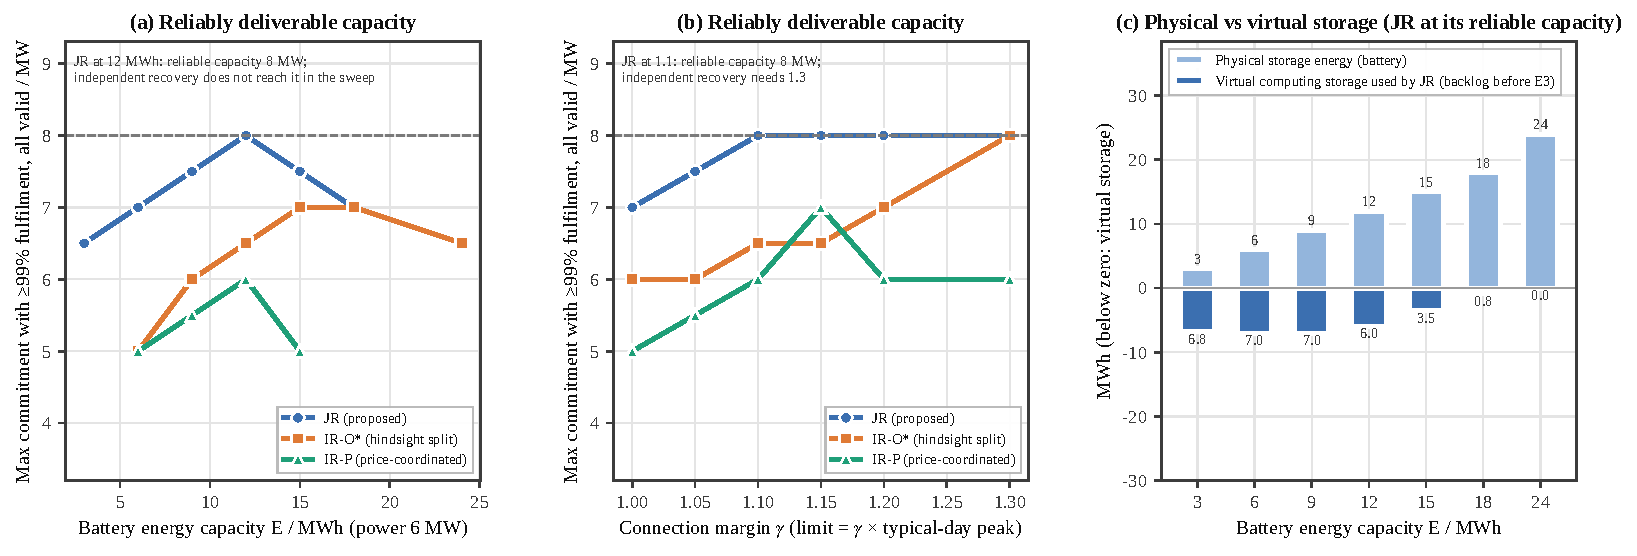
\includegraphics[width=0.96\textwidth]{fig14_substitution.pdf}
\caption{Virtual--physical substitution. (a)(b) Reliably deliverable capacity versus BESS energy and connection margin
(dashed: JR in the base configuration); (c) physical battery energy and the virtual computing storage used by JR
(backlog energy carried into E3) at its reliable capacity.}
\label{fig:subst}
\end{figure*}

Larger batteries are not always better. Beyond 12--15~MWh the reliable capacity of all strategies falls, because in
normal operation a larger battery discharges in the peak-price hours for arbitrage and thereby lowers the
five-day-average baseline: every additional 6~MWh lowers the baseline in the event hours by about 0.6~MW (E1:
10.28~MW with 6~MWh, 8.47~MW with 24~MWh), shrinking the room for reductions measured against it. DR contracts should
therefore consider battery sizing and baseline rules together.

\subsubsection{Shadow prices: scarcity of the recovery channel}
\label{sec:res-price}

With perfect information and a uniform 6~MW, the duals of the joint plan (binaries fixed) reveal the scarcity of the
channel (\tabref{tab:shadow}, \figref{fig:shadow}). Without a rebound charge, the physical connection limit itself
creates competition in the gaps: at $\gamma=1.10$ its shadow price is 1,260--1,455~CNY/MWh (1,771--2,242 at
$\gamma=1.00$), so the channel price is 2.2--3.2 times the peak tariff. With the rebound charge, the binding constraint
becomes the rebound window (3,000~CNY/MWh) and the connection limit is slack. Proposition~\ref{prop:price} is confirmed
numerically: at all interior charging, discharging and catch-up steps of the four settings, the residuals of
$\eta_{\mathrm{c}}\nu_t=\lambda_t+\cdeg$, $\nu_t/\eta_{\mathrm{d}}=\lambda_t-\cdeg$ and $\mu_{c,t}=\varepsilon_t\lambda_t$
are at most $2\times10^{-12}$; for example, $\mu=3.94$~CNY per GPU$\cdot$h in the first gap divided by
$\varepsilon\approx0.99$~kWh per GPU$\cdot$h equals the channel price of about $4.0\times10^3$~CNY/MWh. Long-lag backlog
is the cheapest state: in E3 the marginal cost of C3 backlog (3.19) is well below that of C1 (4.38) because its
deadline lies after E3, so the channel goes first to storage recharging and short-lag catch-up and the long-lag work is
carried across the event, as Theorem~\ref{thm:closed} predicts for several classes.

\begin{table}[!t]
\caption{Shadow prices of the joint plan (CNY/MWh; marginal backlog cost $\mu$ in CNY per GPU$\cdot$h).}
\label{tab:shadow}
\centering\footnotesize
\setlength{\tabcolsep}{3.2pt}
\begin{tabular}{@{}lccccc@{}}
\toprule
Period & $\lambda_t$ & $\lambda^{\mathrm{cap}}_t$ & $\lambda^{\mathrm{rb}}_t$ & $\nu_t$ & $\mu_{1}$ / $\mu_{2}$ / $\mu_{3}$\\
\midrule
\multicolumn{6}{@{}l}{\textit{$\gamma=1.10$, $\crb=3$~CNY/kW}}\\
Gap E1--E2 & 4010 & 0 & 3000 & 4223 & 3.94 / 3.94 / 3.94\\
Gap E2--E3 & 4010 & 0 & 3000 & 4223 & 3.92 / 3.88 / 3.69\\
Event E3 & 4505 & 0 & 0 & 4223 & 4.38 / 3.43 / \textbf{3.19}\\
\multicolumn{6}{@{}l}{\textit{$\gamma=1.10$, $\crb=0$}}\\
Gap E1--E2 & 2464 & \textbf{1455} & 0 & 2657 & 2.49 (all classes)\\
Gap E2--E3 & 2270 & \textbf{1260} & 0 & 2522 & 2.22 (all classes)\\
\multicolumn{6}{@{}l}{\textit{$\gamma=1.00$, $\crb=0$}}\\
Gap E1--E2 & 3252 & \textbf{2242} & 0 & 3285 & 3.16 (all classes)\\
Gap E2--E3 & 2781 & \textbf{1771} & 0 & 3060 & 2.72 (all classes)\\
\bottomrule
\end{tabular}
\end{table}

\begin{figure*}[!t]
\centering
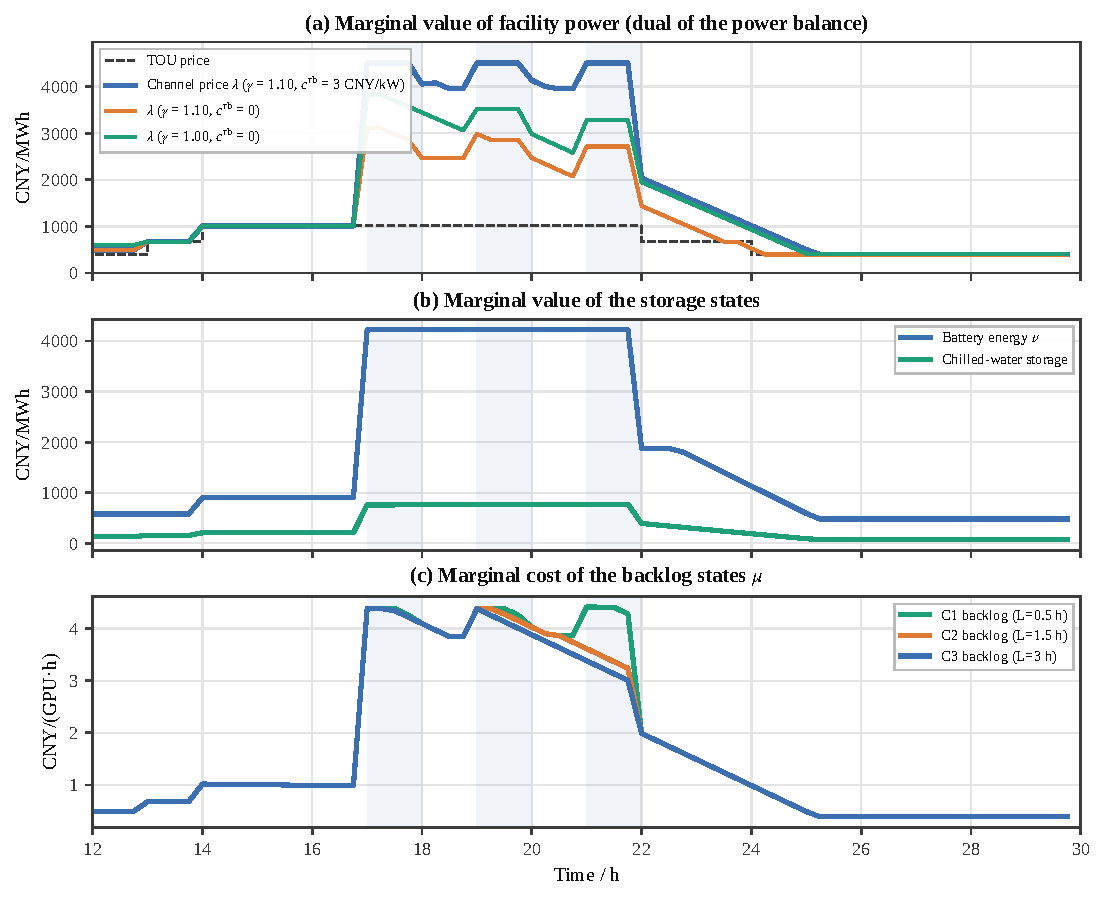
\includegraphics[width=0.80\textwidth]{fig08_shadow_prices.pdf}
\caption{Shadow prices of the joint plan (uniform 6~MW, perfect information). (a) Marginal value of facility electricity
(channel price); (b) marginal value of the storage states; (c) marginal cost of the backlog of each class.}
\label{fig:shadow}
\end{figure*}

\subsubsection{Cross-event capability region}
\label{sec:res-region}

The previous subsections compared strategies for given commitments. When bidding day-ahead, the data center needs to
know which commitment vectors $(C_1,C_2,C_3)$ it can deliver in full. Experiment~25 computes the capability region of
Proposition~\ref{prop:region} under perfect information along 91 rays $C=t\,d$ ($d$ on a simplex grid), together with the
deliverable sets of the benchmarks, the multi-event energy bound and the vertex certificate, for the base case (gap
1~h, $\gamma=1.10$) and a tight case (gap 0.5~h, $\gamma=1.00$). IR-O* uses the hindsight-optimal split for every ray,
the upper limit of any static split (\tabref{tab:region}, \figref{fig:region}).

\begin{table}[!t]
\caption{Capability region of the three events (perfect information).}
\label{tab:region}
\centering\footnotesize
\setlength{\tabcolsep}{1.5pt}
\begin{tabular}{@{}lcc@{}}
\toprule
 & \makecell{Base\\($\tau=1$~h, $\gamma=1.10$)} & \makecell{Tight\\($\tau=0.5$~h, $\gamma=1.00$)}\\
\midrule
Stand-alone capability $\Gamma^0_{1,2,3}$ (MW) & 8.18 / 7.98 / 7.90 & 8.18 / 8.05 / 8.06\\
Support $h_{123}$ of JR (sum of $\Gamma^0_k$) & 24.06 (24.06) & 19.43 (24.29)\\
Energy bound $\bar b$ (MWh) & \makecell{25.66 = 11.36 + 11.41\\ + 9.07 $-$ 6.17} & \makecell{19.57 = 11.58 + 11.40\\ + 2.93 $-$ 6.34}\\
Template $\mathcal T$ & exact (8 vertices) & $\theta^*=0.9997$ (10 vertices)\\
\makecell[l]{Uniform capability (MW):\\JR / IR-P+ / IR-O* / IR-O / IR-P} & \makecell{7.90 / 7.90 / 6.44 /\\ 5.50 / 4.52} & \makecell{6.48 / 6.47 / 6.44 /\\ 3.05 / 2.55}\\
\makecell[l]{Region volume relative to JR:\\IR-P+ / IR-O* / IR-O / IR-P} & \makecell{1.000 / 0.966 /\\ 0.770 / 0.279} & \makecell{0.850 / 0.962 /\\ 0.278 / 0.119}\\
\bottomrule
\multicolumn{3}{@{}p{0.97\columnwidth}@{}}{\scriptsize Energy bound = virtual storage + storage + channel + baseline difference.}
\end{tabular}
\end{table}

\begin{figure*}[!t]
\centering
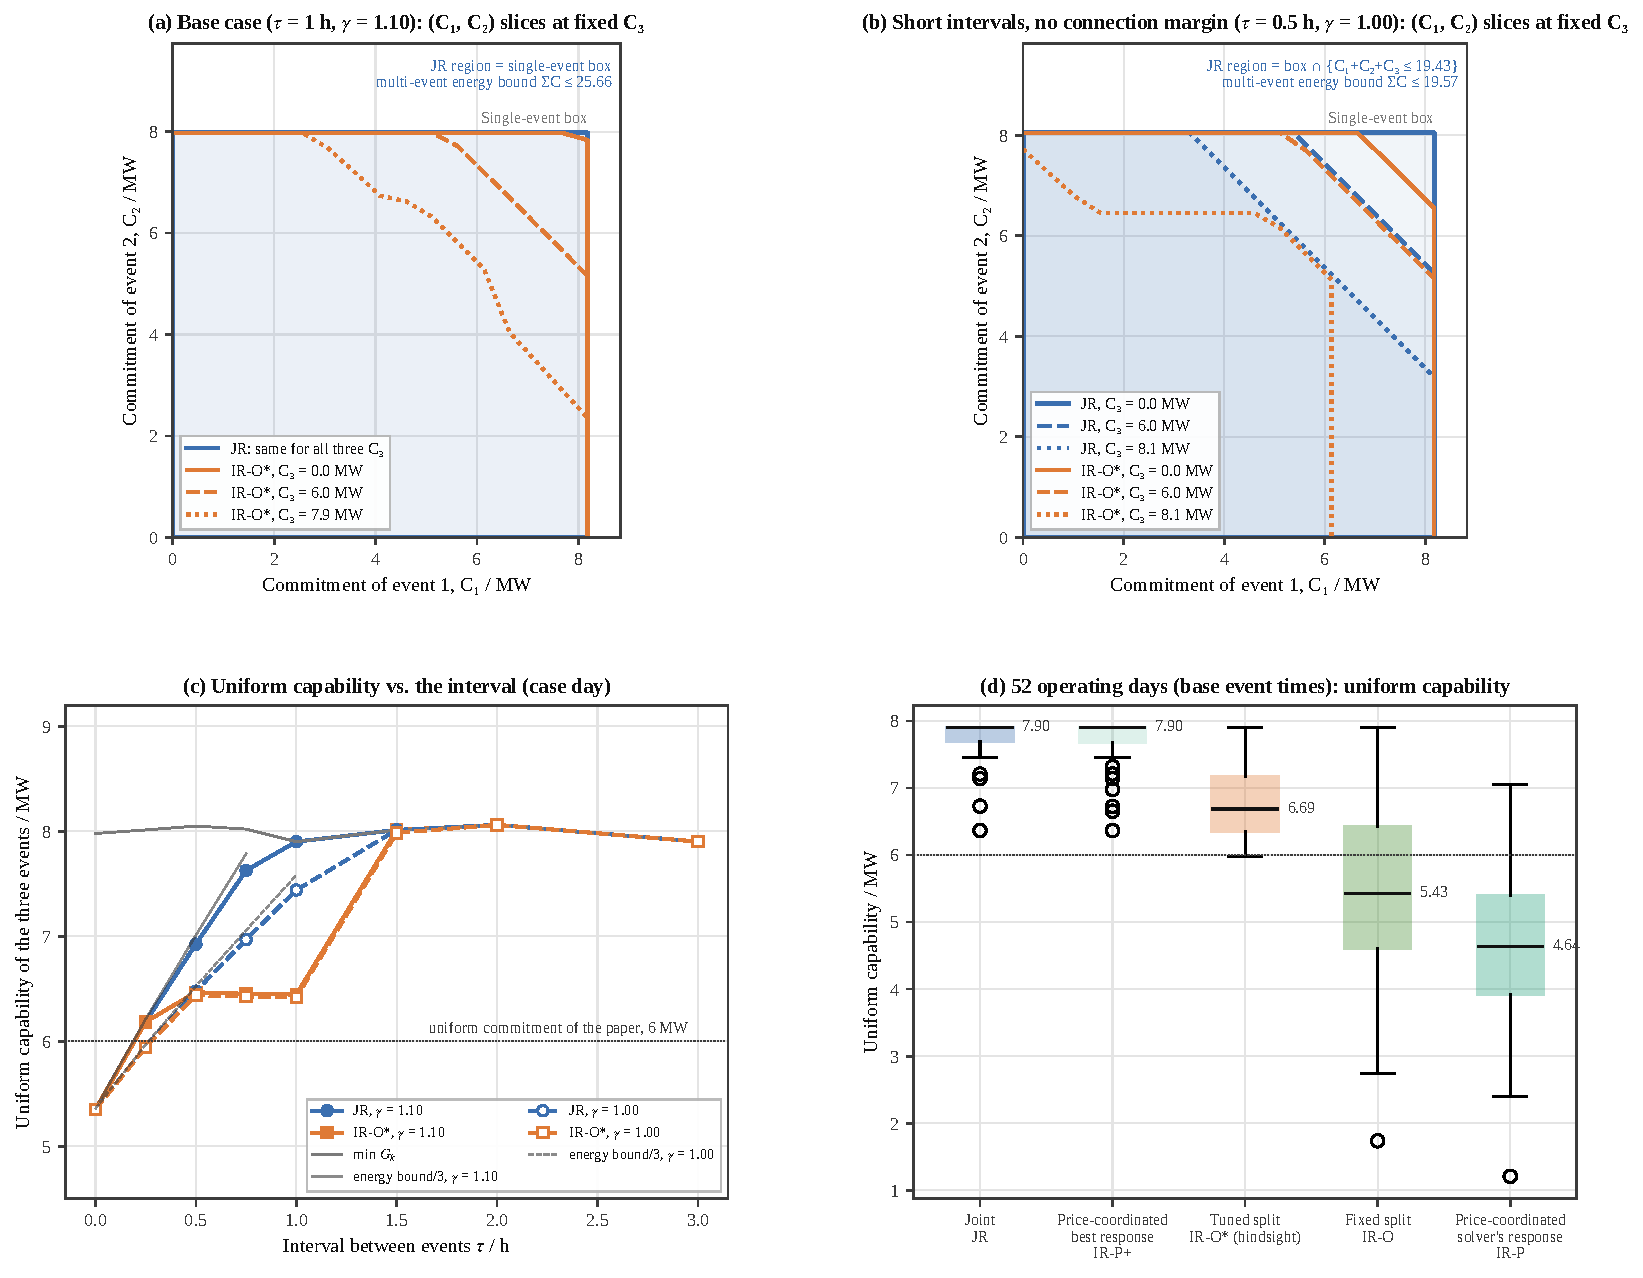
\includegraphics[width=0.86\textwidth]{fig28_region.pdf}
\caption{Cross-event capability region (perfect information). (a)(b) Slices $(C_1,C_2)$ at fixed $C_3$: joint recovery
(shaded, exact by the vertex certificate), IR-O* with the hindsight-optimal split for every commitment vector (lines),
and the single-event box (grey); (c) uniform capability of the three events versus the gap ($\gamma=1.10$ solid, $1.00$
dashed) with the minimum stand-alone capability and one third of the energy bound; (d) uniform capability on the 52
operating days, where IR-P+ is the most favourable and IR-P the solver's response to the price.}
\label{fig:region}
\end{figure*}

The capability region of joint recovery is the single-event box intersected with one total-energy cut. In both cases,
the support of every pair of events equals the sum of their stand-alone capabilities, so two events never conflict;
only the total of the three events can fall below the sum, which gives the single coupling cut $C_1+C_2+C_3\le h_{123}$
(each event lasts 1~h). In the base case, $h_{123}$ equals the sum of the stand-alone capabilities and the region is the
box itself, so the three events are independent; in the tight case the cut removes a corner of the box. This is the
virtual battery of Proposition~\ref{prop:region}: event power limits $\Gamma^0_k$ and one cross-event energy budget
$h_{123}$. All eight vertices of the template are deliverable in the base case, so the description is exact; in the
tight case one vertex falls marginally short ($\theta^*=0.9997$), \ie\ the template differs from the true region by
less than 0.03\%.

The multi-event energy bound is tight: it holds in all 24 gap--margin cases and on all 52 days, and where the cut is
active (14 cases and 18 days) it exceeds the exact LP value by 0.02--0.71~MWh ($\le$3.0\%). On the case day the evening load
without response and storage actions exceeds the baseline by about 2.2~MW, so the baseline difference $\Delta$ of the three events
is $-6.2$ to $-6.7$~MWh for gaps up to 1~h, a non-negligible part of the budget that the unbiased-baseline assumption
of Proposition~\ref{prop:bound} would ignore (the bound would overestimate by 42\% at a zero gap).

Independent recovery shrinks the cross-event energy budget rather than the stand-alone capabilities. In the base case
IR-O* reaches the JR boundary in every single-event and two-event direction, and the loss concentrates in the corner
where all three commitments are high: the maximum total commitment along the same rays is 19.33 against 23.70~MW
($-18.4\%$) and the uniform capability 6.44 against 7.90~MW ($-18.4\%$), although the volume is only 3.4\% smaller. The
fixed split IR-O loses more (volume $-23\%$, uniform capability 5.50~MW). In the tight case the channel is narrow
anyway and IR-O* nearly coincides with JR (Corollary~\ref{cor:novalue}(c)), but in directions with only two committed
events it still loses up to 11\%.

A price signal alone is not enough. The optimal IT response to the channel price is not unique, and the response
picked by the solver (IR-P) delivers only 53--82\% of JR along the rays of the base case (28\% of the volume) and 60\%
of the uniform capability of JR on average over the 52 days. Selecting the most favourable exactly optimal response
(IR-P+) reaches the JR boundary on all rays of the base case but only on 59\% of the rays of the tight case; with
$\gamma=1.00$ and gaps of 1.5--3~h no exactly optimal response is deliverable (uniform capability 4.97--5.72~MW against
7.90--8.06~MW for JR). Allowing the IT side to be 0.1\% suboptimal recovers the JR capability in all 24 cases and on all
52 days, except for up to 5\% in some directions of the tight case; the residual gap arises because the IT model
estimates its power budget with idle storage and converts cooling with the electric-chiller COP, so the joint price is
only an approximate supporting price for it. The channel price thus contains almost all the information needed but
does not select a deliverable plan: the IT side must also know which of its many near-optimal plans to choose.

The uniform capability of JR increases almost linearly with the gap and follows the energy bound
(\figref{fig:region}(c)). At a zero gap, JR, IR-O* and IR-P+ coincide (5.35~MW), since nothing can be recovered between
the events. JR reaches the stand-alone capability at a gap of 1~h with $\gamma=1.10$ and 1.5~h with $\gamma=1.00$; at a
gap of 1~h its uniform capability is 7.44/7.88/7.90~MW for $\gamma$ = 1.00/1.05/1.10. IR-O* stays at about 6.4~MW for gaps
of 0.5--1~h, because it spends the channel on unnecessary catch-up, and catches up with JR only from 1.5~h, which is the
difference of the minimum recovery gaps of Theorem~\ref{thm:closed} on the capability region. Over the 52 days the
uniform capability of JR averages 7.75~MW (6.37--7.90); relative to JR, IR-P+ achieves 99.4\%, IR-O* 88.6\% (80--100\%),
IR-O 71\% and IR-P 60\%, and the energy cut is active on 18 days.

For bidding, the current practice of one value per event requires the uniform capability to guarantee delivery under
any call pattern: 7.90~MW per event in the base case and 6.48~MW in the tight case. If the data center instead declares
the virtual-battery parameters (three $\Gamma^0_k$ and the budget $h_{123}$, four numbers), the grid operator may call
any combination within them; in the tight case, two calls of up to 8.0~MW each become possible, 24\% more than the
uniform declaration, while three calls may total at most 19.43~MW. Under independent recovery the same declaration
needs a further discount: the energy budget of IR-O* is 18\% lower than that of JR in the base case.

\subsubsection{Distributed coordination by plan--price exchange}
\label{sec:res-admm}

The previous subsection showed that a one-shot channel price does not determine a deliverable plan. Experiment~26 lets
the IT scheduler and the facility controller keep their own models, states and forecasts and exchange only the
deferrable power plan (one number per step) and the price, iterating \eqref{eq:admm} on the same joint model
(Proposition~\ref{prop:admm}); the facility side requires every called event to be valid and $\rho=200$~CNY per
MW$^2$ and step unless stated otherwise (\figref{fig:admm}).

\begin{figure*}[!t]
\centering
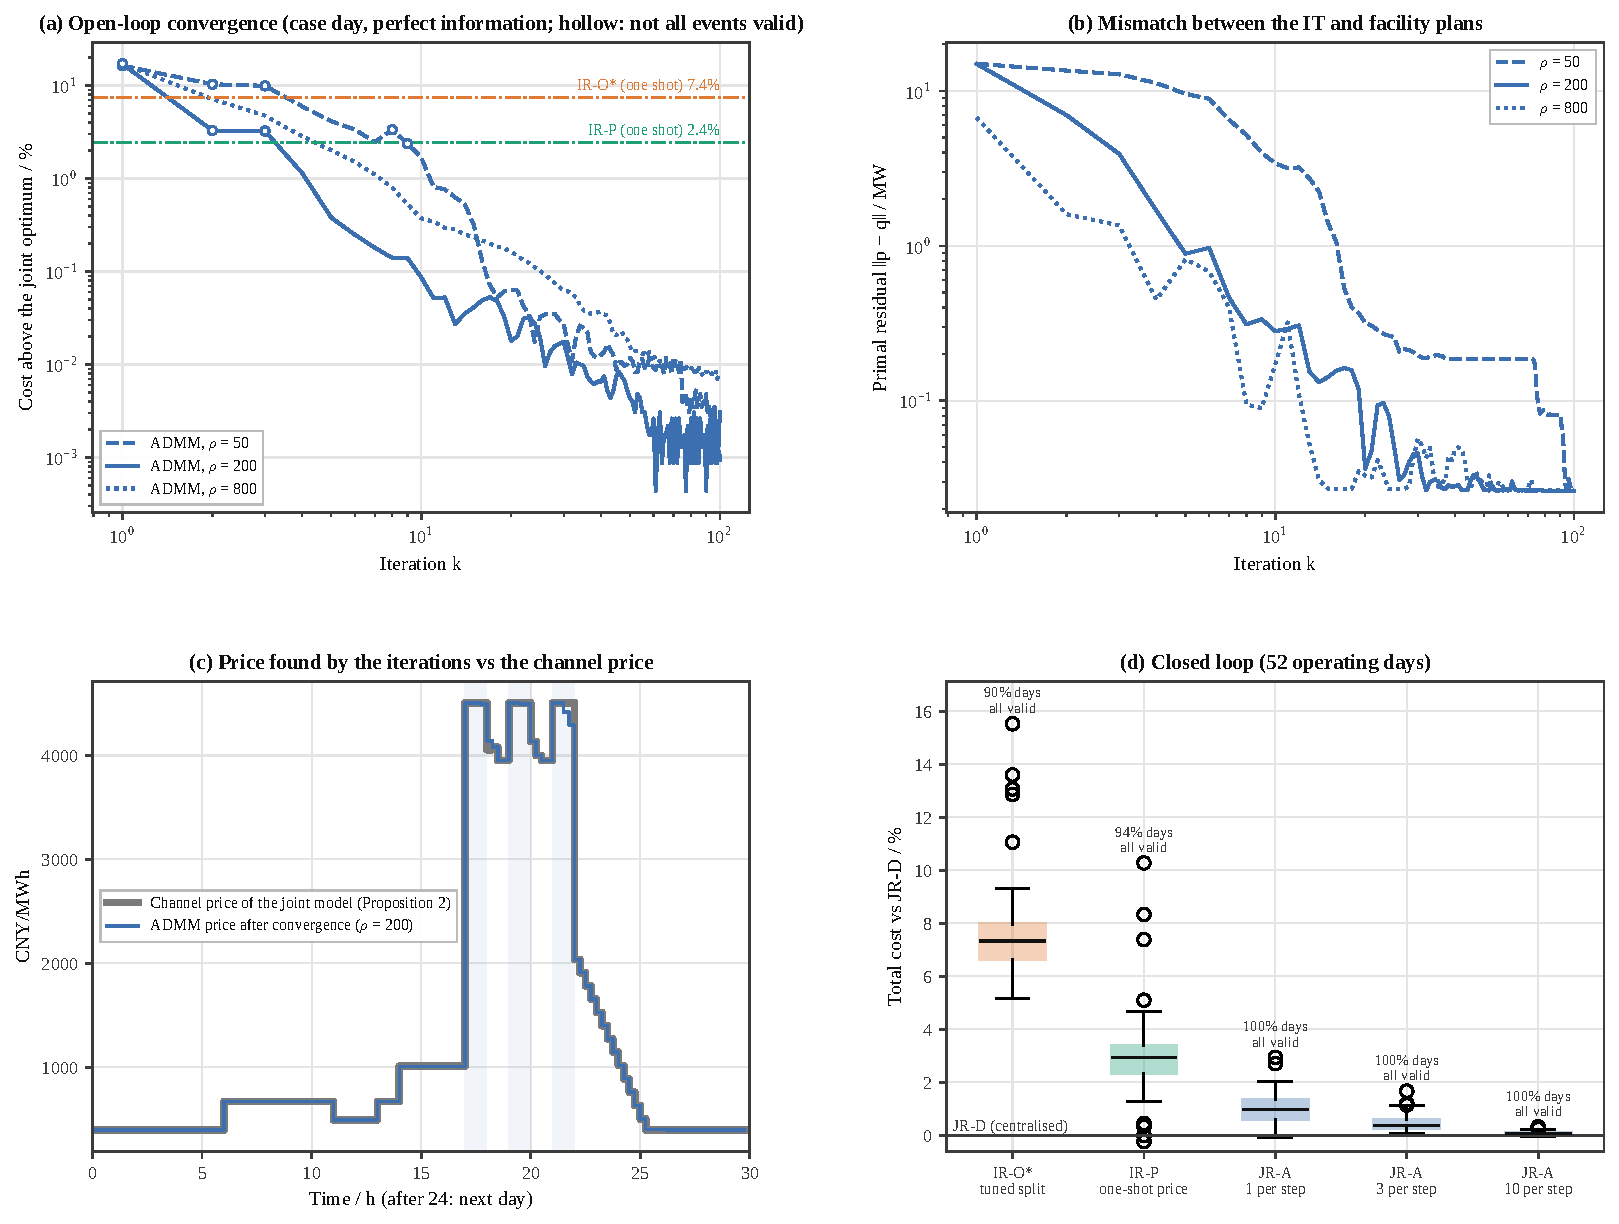
\includegraphics[width=0.86\textwidth]{fig29_admm.pdf}
\caption{Distributed joint recovery by plan--price exchange. (a) Open-loop cost of implementing the IT side's plan
relative to the joint optimum (log--log; hollow: not all events valid), with the one-shot benchmarks IR-P and IR-O*;
(b) mismatch between the two plans; (c) price after convergence ($\rho=200$) and channel price of the joint model
(shaded: events); (d) closed-loop cost relative to the centralised JR-D on 52 operating days and share of days with all
events valid.}
\label{fig:admm}
\end{figure*}

In open loop (case day, perfect information, uniform 6~MW), the relevant measure is the cost of implementing the IT
side's current plan, \ie\ the total cost when the facility responds optimally to it. With $\rho=200$ this cost falls
below that of the one-shot price coordination IR-P (2.44\% above the joint optimum) from the fourth iteration on, and
lies 0.38\%, 0.09\% and 0.02\% above the optimum after 5, 10 and 20 iterations; IR-O* with the hindsight-optimal split
is 7.38\% above. The iteration starts from the nominal IT load, and the IT plans of the first three iterations do not yet
keep all events valid: a few exchanges are needed to move catch-up out of the scarce hours. A small $\rho$ updates the
price slowly ($\rho=50$: better than IR-P from iteration 10, within 0.1\% from iteration 17), and a large one locks
the plans early ($\rho=800$: iterations 5 and 26). After 100 iterations the residual stays at about 0.03~MW, the
resolution of the tangent cuts, and the implemented cost is within 0.001--0.008\% of the optimum.

The price found by the iteration is the channel price (\figref{fig:admm}(c)). After convergence it differs from the
channel price of the joint model (Proposition~\ref{prop:price}) by less than 1~CNY/MWh in 79\% of the steps, and it
reproduces the price of about 4,500~CNY/MWh during the events and its gradual decline afterwards; only three steps at
the beginning and end of the events differ more (up to 214~CNY/MWh). The iteration discovers the channel price without
any party solving the joint model and broadcasting it.

In closed loop, the centralised JR-D costs $22.84\times10^4$~CNY on the case day, and JR-A with 1, 3 and 10 iterations
per MPC step costs $+0.67\%$, $+0.22\%$ and $+0.03\%$ more; with three iterations, $\rho$ = 50, 200 and 800 differ by
less than 0.1\%. Over the 52 days, JR-A costs $+0.99\%$, $+0.45\%$ and $+0.09\%$ more than JR-D with 1, 3 and 10
iterations and keeps all events valid on every day, whereas IR-P costs $+2.97\%$ more (all events valid on 94\% of the
days). One exchange per step thus recovers 67\% of the advantage of joint recovery over the strongest independent
benchmark, three exchanges 85\% and ten 97\%. A full day takes about 6~s for JR-D and 12/29/88~s for JR-A with
1/3/10 iterations, less than 1~s per step. Joint recovery therefore does not require merging the IT scheduler and the
facility energy management system: both keep their own models and data, provided that plans and prices are exchanged in
both directions a few times per 15~min.
